\section{ETHICS ASPECTS}

According to the article 8 of the Charter of Fundamental Rights of the European Union: ``Everyone has the right to the protection of personal data concerning him or her''. 
Concerning this fact, the present project has a potentially sensitive issue, as the collected data comes from real patients suffering prostate cancer.
It is important to stress that the participants of the database are fully informed of the aims and uses of the \ac{mri} images, and a signature is required for consent.
But more importantly, \emph{no personal data is used or available} in this project, as every image is thoroughly anonymized before the data is transferred to processing for research. 

\newpage

\section{LETTER OF COMMITMENT OF PARTNER ORGANISATION}

\begin{figure}[!h]
  \centering
  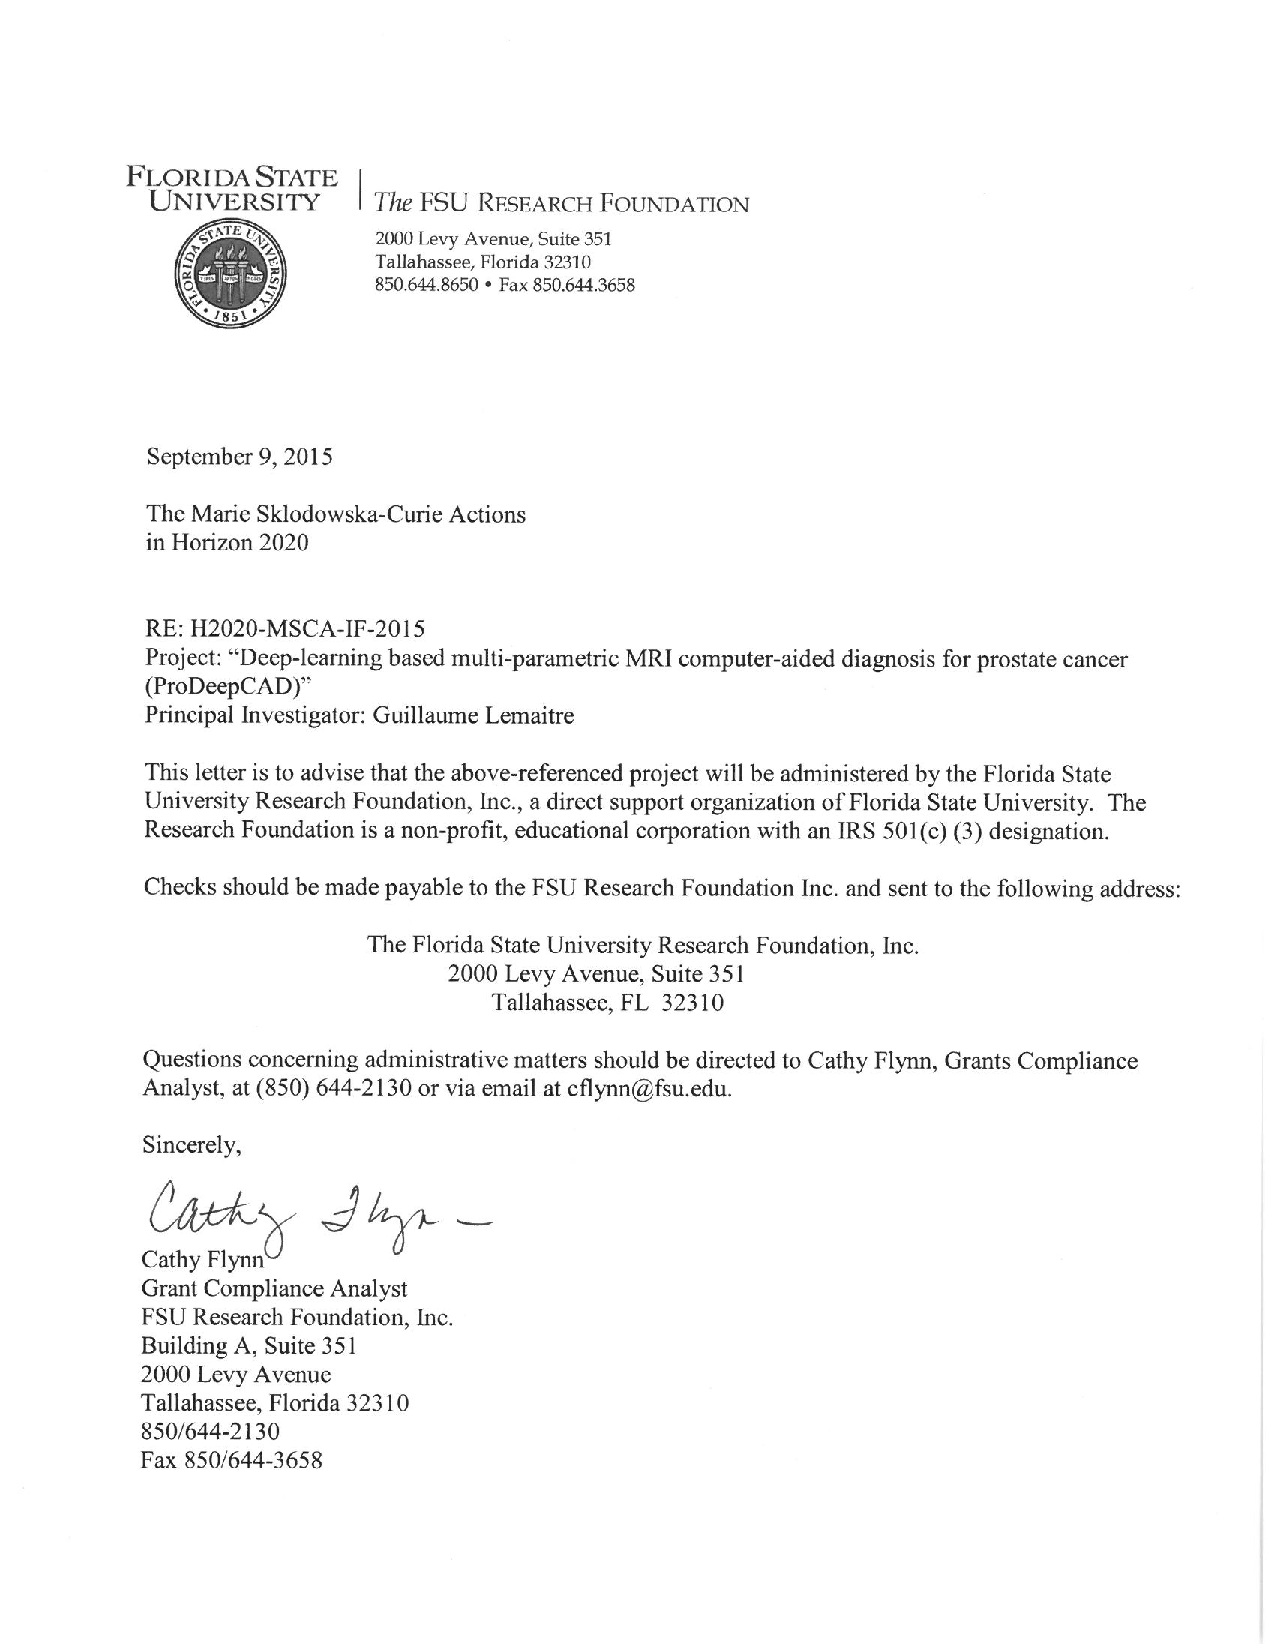
\includegraphics[height=.96\textheight]{./content/ethical/lemaitre.pdf}
\end{figure}
